\documentclass[12pt,xcolor=dvipsnames]{beamer}
\usetheme{CambridgeUS}
\usecolortheme{whale}
\setbeamercolor{block title}{use=structure,fg=white,bg=blue!75!black}  
\setbeamercolor{block body}{use=structure,fg=black,bg=blue!5!white}
\setbeamercolor{frametitle}{bg=Blue}

\usepackage{hyperref}   
\usepackage{url}
\hypersetup{urlcolor=red}

\renewcommand{\bibname}{References}
\setbeamertemplate{bibliography item}{[\theenumiv]}

\usepackage{multicol}
\usepackage{multirow}
\usepackage{verbatim} 
\usepackage{graphics}
\usepackage{graphicx}


\usepackage{chapterbib}
%\usepackage{tikz}
%\usepackage{pgfplots}
%\usepgfplotslibrary{groupplots} 
%\usepackage{pgf, pgfarrows, pgfnodes}
\usepackage{lscape}
\usepackage{longtable}
\usepackage{float}
\usepackage{url}
\usepackage{multicol}
\usepackage{color}
\usepackage{multirow}
\usepackage{listings}
\usepackage{subfigure}
\usepackage{tabularx,ragged2e,booktabs,caption}
\usepackage{placeins}
\usepackage[toc,page]{appendix}


%Basic Information
\title{Load Testing and Benchmarking for BigData}
\author{Aayush Agrawal, Sunil Raiyani, Jayam Modi}

%--------------------------------------------------------------------------------------
%               TITLE PAGE (Slide 1)
%--------------------------------------------------------------------------------------
\begin{document}
 


\begin{frame}
\titlepage
\end{frame}
%--------------------------------------------------------------------------------------


%--------------------------------------------------------------------------------------
%               Outline
%--------------------------------------------------------------------------------------
%\begin{frame}
%\frametitle{Outline}
%\begin{multicols}{2}
%\tableofcontents[hideallsubsections]
%\end{multicols}
%\end{frame}

%--------------------------------------------------------------------------------------
%               Slide 1: Topic 1
%--------------------------------------------------------------------------------------

\begin{frame}[t]
\frametitle{Aim of the Project}
The aim of the project is Load Testing and Benchmarking for BigData. 
\newline
\newline
The major task is to setup a distributed file system on a cluster, test the data and query processing capacity 
of the system using BigBench and predict the performance of the system for larger data sets.
\end{frame}










\begin{frame}[t]
\frametitle{Block Diagram}
\begin{figure}[h]
 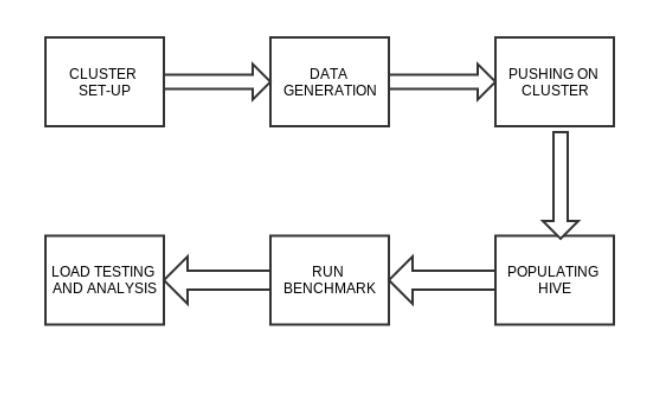
\includegraphics[width=10cm]{block_diagram.jpeg}
\caption{Average Query Response Times for different data sizes \label{block}}
\end{figure}
\end{frame}

\section{Achievements}
\begin{frame}[t]
\frametitle{Achievements}
\begin{enumerate}
 \item Customized version of BigBench.\cite{bigbenchgit} 
 \item Evaluating factors affecting the average query response time on the cluster.
\end{enumerate}




\end{frame}




\section{Future Scope}
\begin{frame}[t]
\frametitle{Future Scope}
 The following work is considered for future:
\begin{itemize}
 \item  Run the experiment for clusters of larger size and try to determine the optimum size of cluster of the given
	configuration of nodes to manage a particular data-set size.
 \item Analyze other parameters affecting the average query response time of the system.
 \item  Open Source Release of our customized version of BigBench.\cite{bigb}
\end{itemize}
\end{frame}





















%---------------------------------------------------------------------------------------
%     Final Slide - References
%--------------------------------------------------------------------------------------
\section{References }
\frametitle{References }
\begin{frame}[allowframebreaks]{References}
\bibliographystyle{ieeetr}
\bibliography{biblio}





\end{frame}
\end{document}
